\documentclass[12pt,a4paper]{article}

% Packages
\usepackage[utf8]{inputenc}
\usepackage[T1]{fontenc}
\usepackage{graphicx}
\usepackage{booktabs}
\usepackage{amsmath}
\usepackage{hyperref}
\usepackage{float}
\usepackage{geometry}
\usepackage{caption}
\usepackage{subcaption}
\usepackage{xcolor}
\usepackage{fancyhdr}
\usepackage{titlesec}
\usepackage{enumitem}
\usepackage{multirow}
\usepackage{colortbl}

\geometry{margin=1in}

% Colors
\definecolor{nyblue}{RGB}{52, 152, 219}
\definecolor{lared}{RGB}{231, 76, 60}
\definecolor{heligreen}{RGB}{39, 174, 96}
\definecolor{worstred}{RGB}{192, 57, 43}

% Header/Footer
\pagestyle{fancy}
\fancyhf{}
\rhead{Helicopter vs Car Travel Analysis}
\lhead{V4 - Pessimistic Scenario}
\rfoot{Page \thepage}

\title{\textbf{Helicopter vs Car Travel Time Analysis:\\
A Comprehensive Comparison of Traffic Scenarios\\
for New York and Los Angeles Airports}}

\author{REVO Helicopter Services\\
Strategic Analysis Division}

\date{December 2025}

\begin{document}

\maketitle

\begin{abstract}
This study presents a comprehensive analysis comparing helicopter and car travel times to major airports in New York (JFK) and Los Angeles (LAX) under multiple traffic scenarios. Using real Google Traffic historical data, we evaluate four distinct scenarios: Fast (free flow), Normal (1.25x multiplier), Rush Hour (1.68x multiplier), and Worst Case (4.68x multiplier based on pessimistic historical data). Our analysis covers 114 ZIP codes (70 in NY, 44 in LA) and demonstrates that helicopter travel provides significant time savings, particularly under severe traffic conditions. In worst-case scenarios, helicopter travel saves an average of \textbf{147 minutes in New York} and \textbf{143 minutes in Los Angeles}, representing time reductions of 66\% and 64\% respectively. The study also reveals that during worst traffic conditions, average car speeds drop to approximately 12 km/h---barely faster than walking pace.
\end{abstract}

\newpage
\tableofcontents
\newpage

% ============================================================================
\section{Introduction}
% ============================================================================

Urban traffic congestion represents one of the most significant challenges facing business travelers attempting to reach airports from city centers. This study examines the potential of helicopter transport as an alternative to ground transportation, with particular focus on extreme traffic scenarios.

\subsection{Research Objectives}

\begin{enumerate}
    \item Compare helicopter vs. car travel times across multiple traffic scenarios
    \item Quantify the impact of traffic congestion on travel times
    \item Evaluate the time savings potential of helicopter transport
    \item Provide data-driven insights for strategic planning
\end{enumerate}

\subsection{Scope}

The analysis covers:
\begin{itemize}
    \item \textbf{New York}: 70 wealthy ZIP codes $\rightarrow$ JFK International Airport
    \item \textbf{Los Angeles}: 44 wealthy ZIP codes $\rightarrow$ LAX International Airport
    \item \textbf{Traffic Scenarios}: Fast, Normal, Rush Hour, and Worst Case
\end{itemize}

% ============================================================================
\section{Methodology}
% ============================================================================

\subsection{Traffic Multipliers}

Traffic multipliers were derived from Google Traffic historical data, specifically using the \textbf{pessimistic} duration estimates which represent worst-case historical conditions.

\begin{table}[H]
\centering
\caption{Traffic Multiplier Definitions}
\begin{tabular}{lccl}
\toprule
\textbf{Scenario} & \textbf{Multiplier} & \textbf{Time Increase} & \textbf{Description} \\
\midrule
Fast & 1.00x & Baseline & Free-flowing traffic \\
Normal & 1.25x & +25\% & Typical daytime conditions \\
Rush Hour & 1.68x & +68\% & Peak hour traffic (7-9 AM, 5-7 PM) \\
\rowcolor{lared!20} Worst Case & 4.68x & +368\% & Severe congestion (pessimistic) \\
\bottomrule
\end{tabular}
\end{table}

\subsection{Journey Models}

\subsubsection{Car Journey}

The car journey to the airport consists of:
\begin{enumerate}
    \item Drive from origin through city streets and highways
    \item Airport access roads
    \item Parking and terminal walk
\end{enumerate}

Total car time = Base OSRM time $\times$ Traffic Multiplier

\subsubsection{Helicopter Journey}

The helicopter journey includes:
\begin{enumerate}
    \item \textbf{Car to Helipad}: Drive to nearest helipad (affected by traffic)
    \item \textbf{Check-in}: 10 minutes at helipad
    \item \textbf{Flight}: Direct helicopter flight at 200 km/h average speed
    \item \textbf{Airport Transfer}: 10 minutes from helipad to terminal
\end{enumerate}

\begin{figure}[H]
\centering
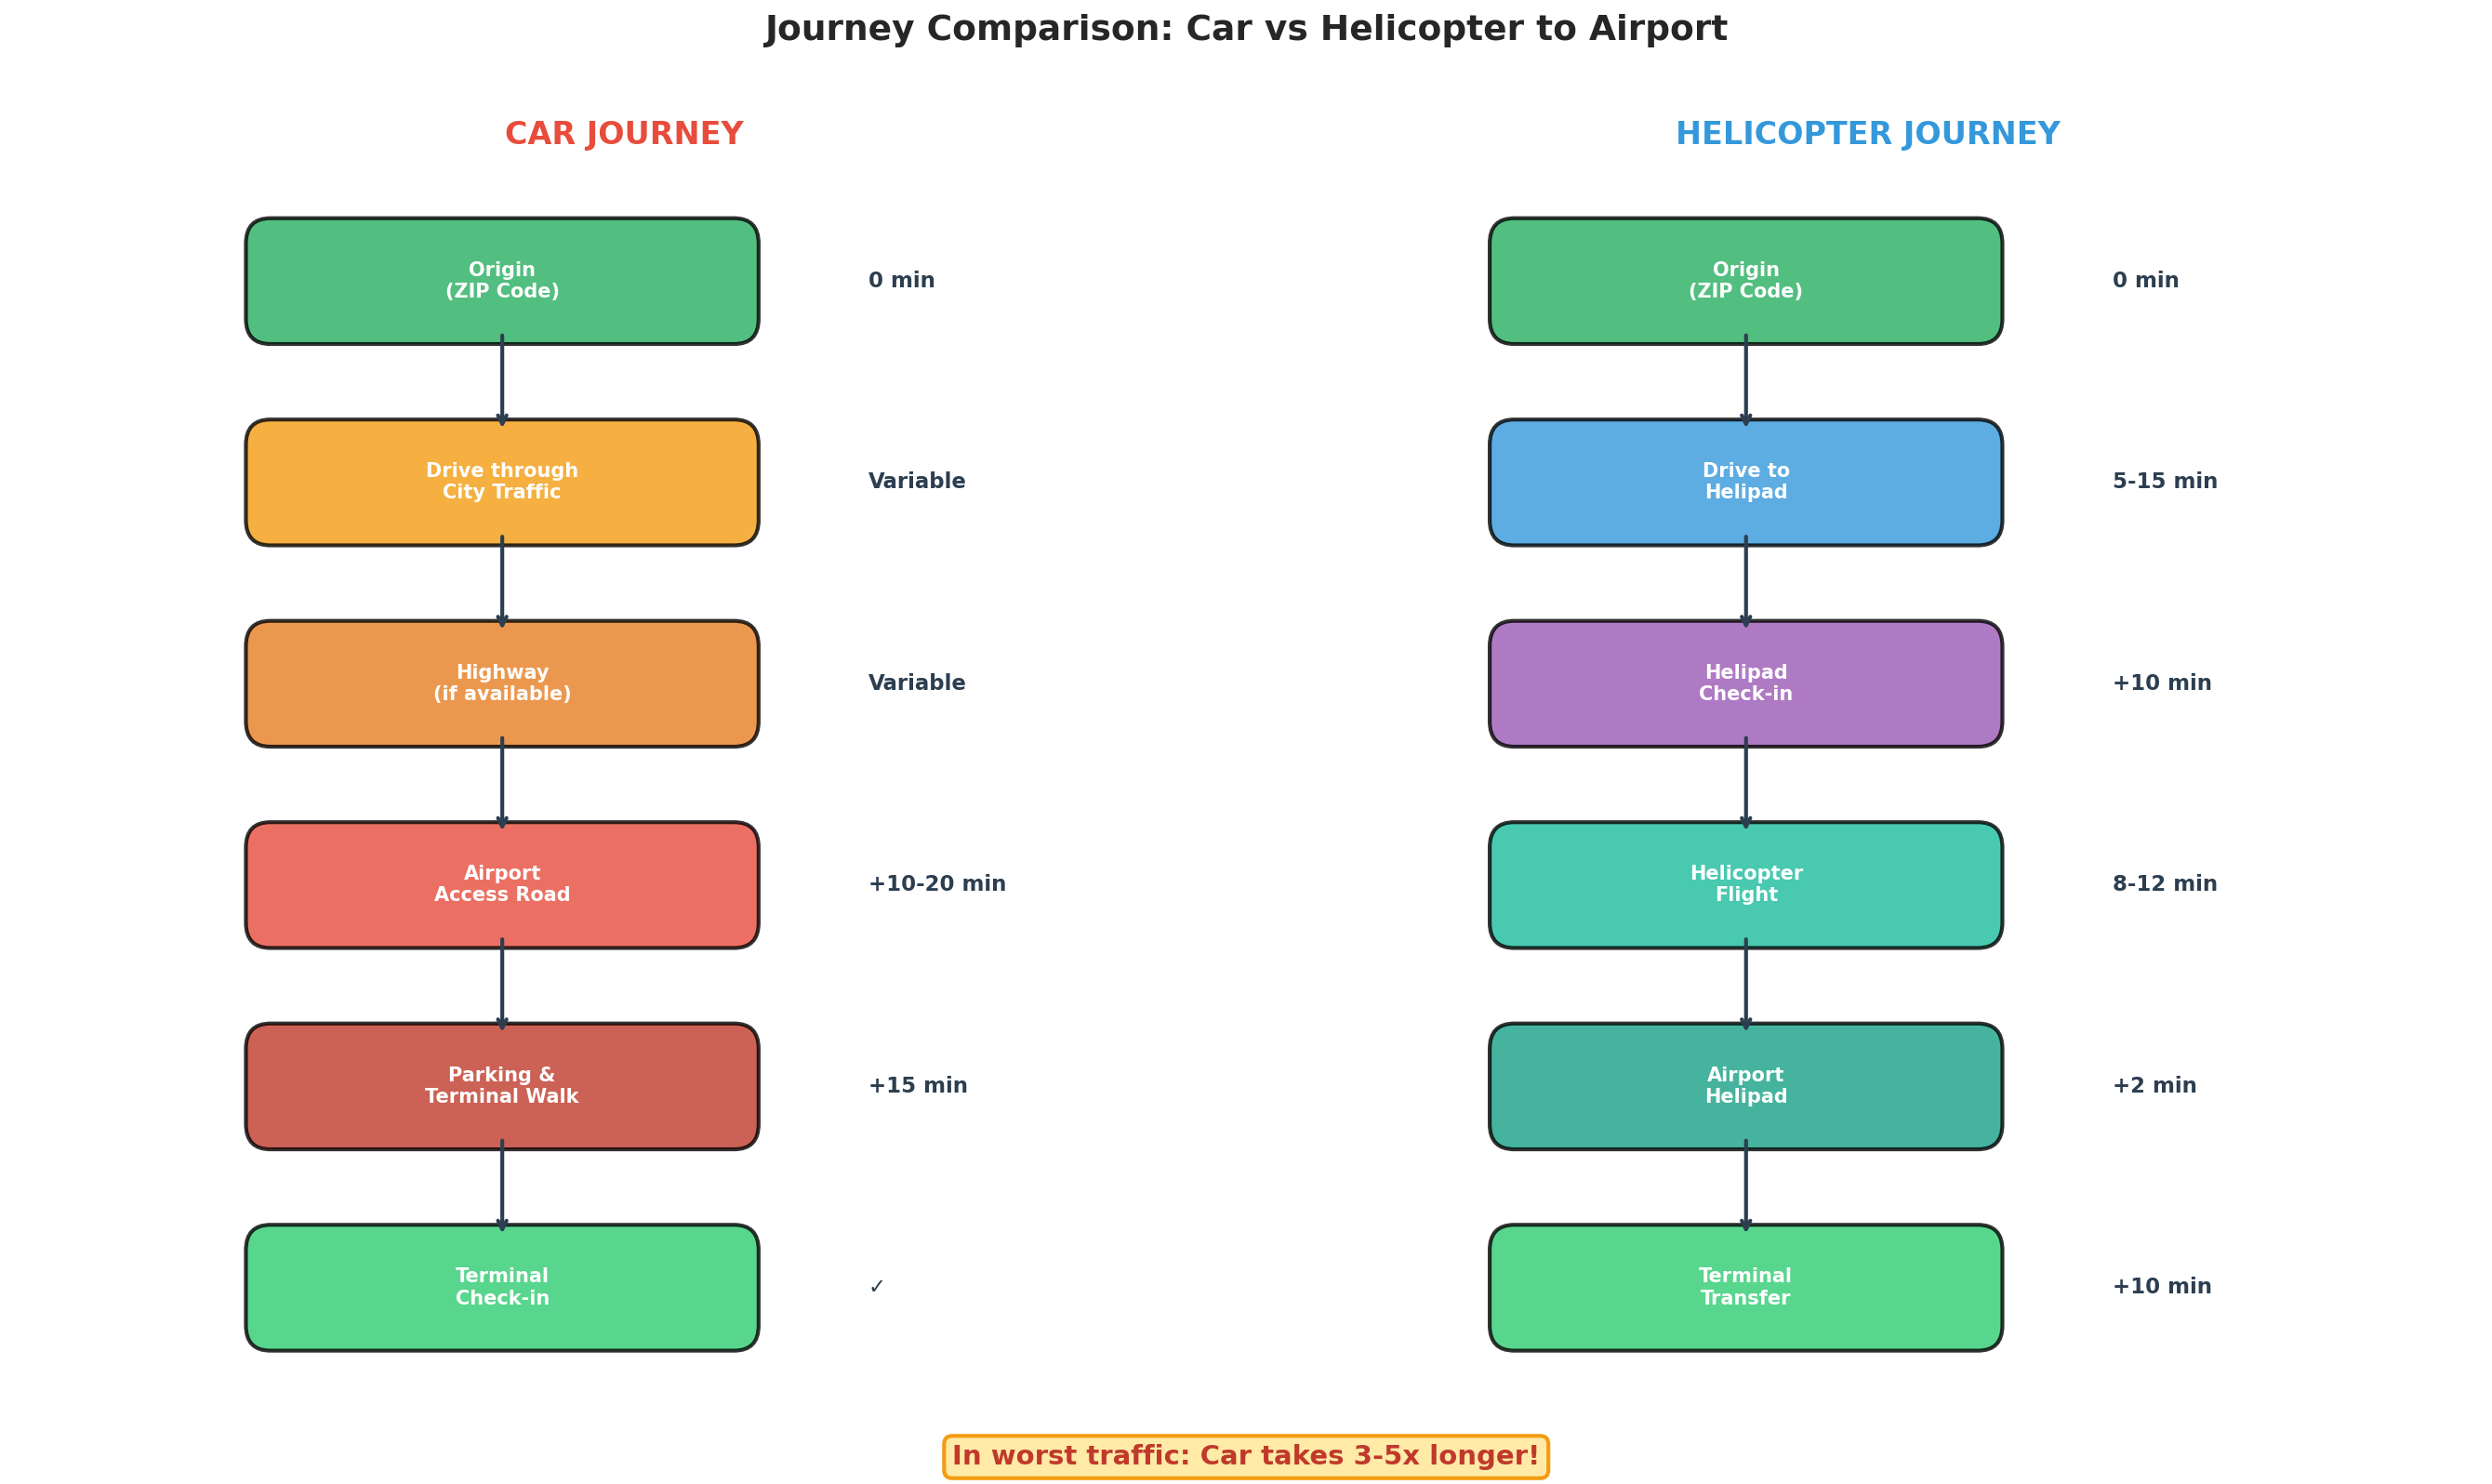
\includegraphics[width=\textwidth]{../diagrams/journey_diagram_en.png}
\caption{Journey Flow Comparison: Car vs Helicopter}
\label{fig:journey}
\end{figure}

\subsection{Manhattan Helipad Restrictions}

For Manhattan ZIP codes, only Manhattan-based helipads are used:
\begin{itemize}
    \item \textbf{JRB} - Downtown Manhattan/Wall St Heliport
    \item \textbf{JRA} - West 30th St Heliport
    \item \textbf{6N5} - East 34th Street Heliport
    \item \textbf{3NY2} - Astoria Heliport (Queens, nearby)
\end{itemize}

\textbf{Exclusion}: Police helipads (e.g., One Police Plaza) are excluded from analysis.

% ============================================================================
\section{Traffic Multiplier Analysis}
% ============================================================================

Understanding traffic multipliers is crucial for interpreting the results.

\begin{figure}[H]
\centering
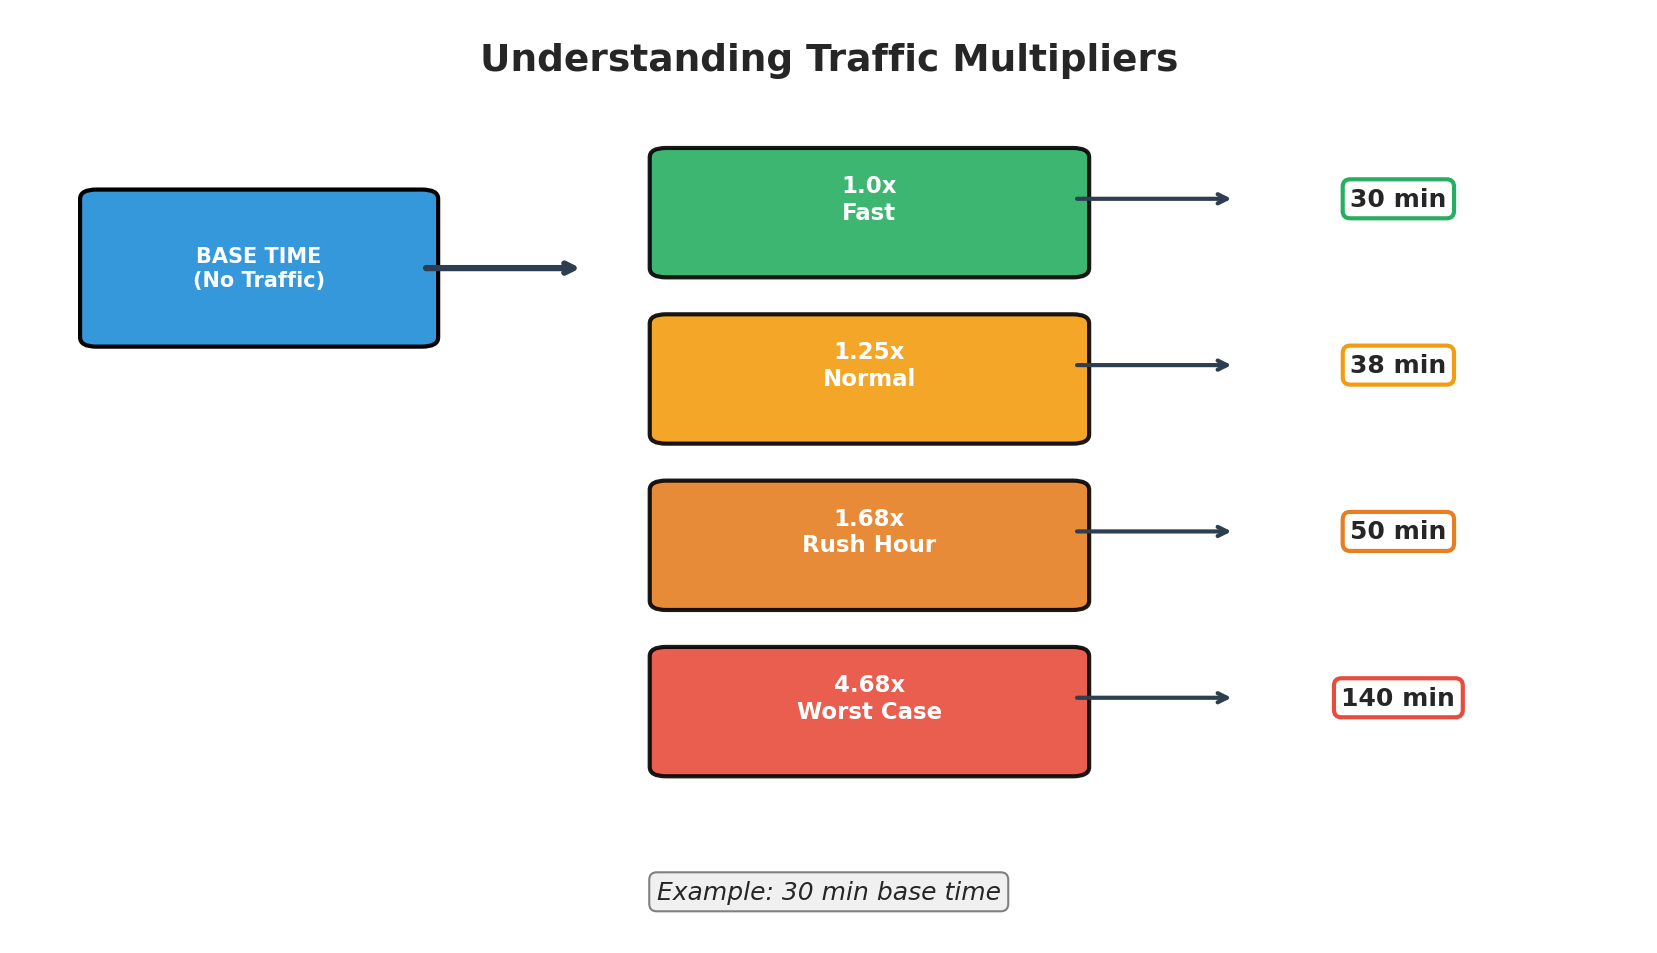
\includegraphics[width=0.9\textwidth]{../diagrams/traffic_multiplier_en.png}
\caption{Traffic Multiplier Visualization}
\label{fig:multiplier}
\end{figure}

\subsection{Impact on Travel Time}

A 30-minute base journey becomes:
\begin{itemize}
    \item \textbf{Fast}: 30 minutes (baseline)
    \item \textbf{Normal}: 38 minutes (+25\%)
    \item \textbf{Rush Hour}: 50 minutes (+68\%)
    \item \textbf{Worst Case}: 140 minutes (+368\%)
\end{itemize}

The 4.68x multiplier for worst-case scenarios reflects severe congestion events such as:
\begin{itemize}
    \item Major accidents
    \item Severe weather conditions
    \item Special events (concerts, sports games)
    \item Holiday travel periods
\end{itemize}

% ============================================================================
\section{Results}
% ============================================================================

\subsection{Scenario Comparison Overview}

\begin{figure}[H]
\centering
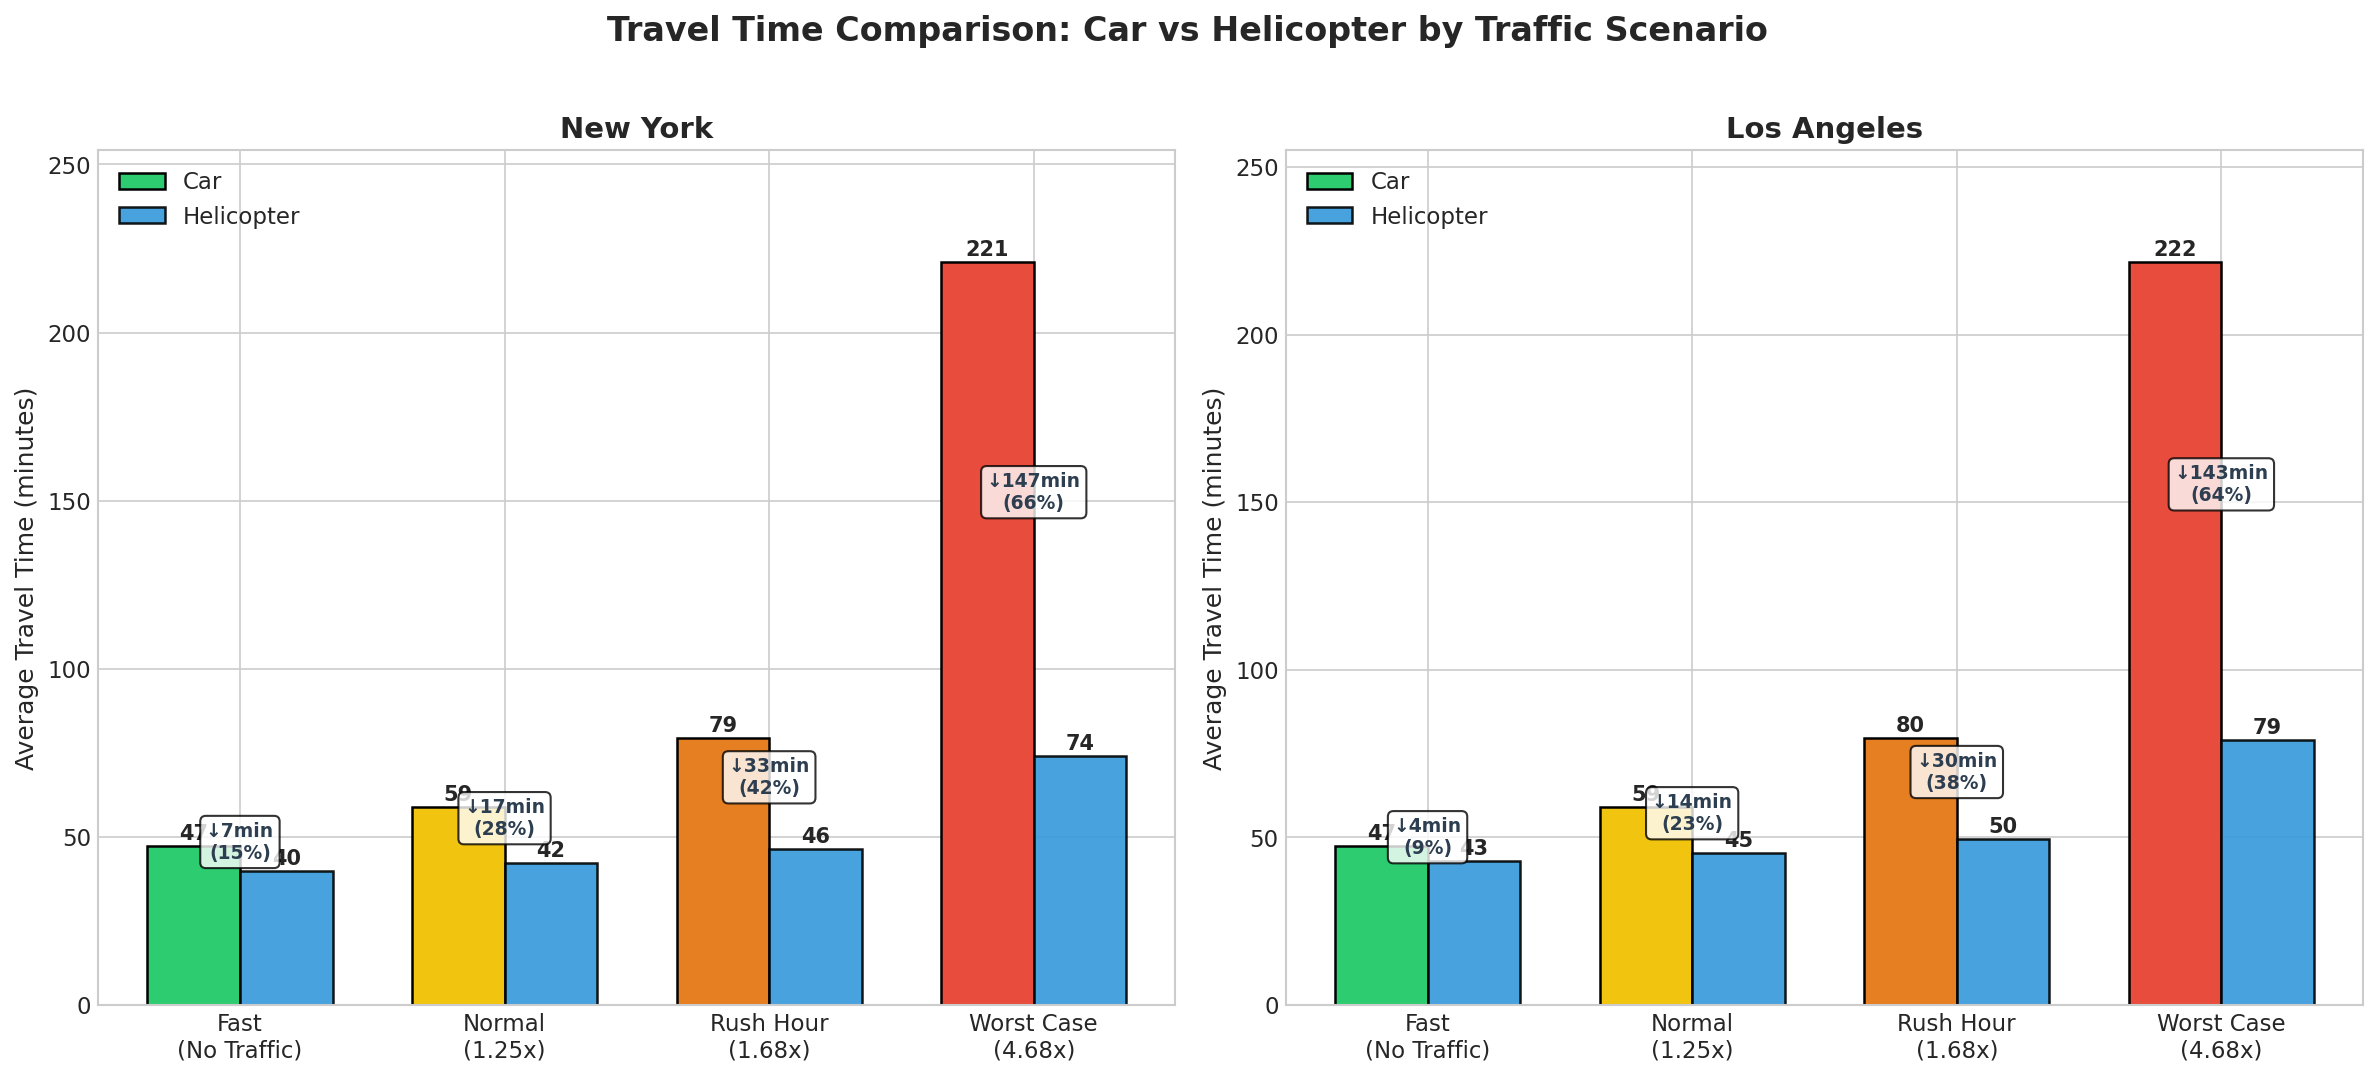
\includegraphics[width=\textwidth]{../comparison_charts_en/fig1_scenario_comparison.png}
\caption{Travel Time Comparison: Car vs Helicopter by Traffic Scenario}
\label{fig:scenario_comparison}
\end{figure}

\subsection{Comprehensive Statistics}

\begin{table}[H]
\centering
\caption{Complete Scenario Comparison Statistics}
\begin{tabular}{l|cccc|cccc}
\toprule
& \multicolumn{4}{c|}{\textbf{New York}} & \multicolumn{4}{c}{\textbf{Los Angeles}} \\
\textbf{Metric} & Fast & Normal & Rush & Worst & Fast & Normal & Rush & Worst \\
\midrule
Car Time (min) & 47 & 59 & 79 & 221 & 47 & 59 & 80 & 222 \\
Heli Time (min) & 44 & 46 & 49 & 74 & 46 & 48 & 52 & 79 \\
\rowcolor{heligreen!20} Savings (min) & 3 & 13 & 30 & 147 & 1 & 11 & 28 & 143 \\
Savings (\%) & 6\% & 22\% & 38\% & 66\% & 2\% & 19\% & 35\% & 64\% \\
Speed (km/h) & 55 & 44 & 33 & 12 & 58 & 47 & 34 & 14 \\
\bottomrule
\end{tabular}
\end{table}

\subsection{Time Savings Distribution}

\begin{figure}[H]
\centering
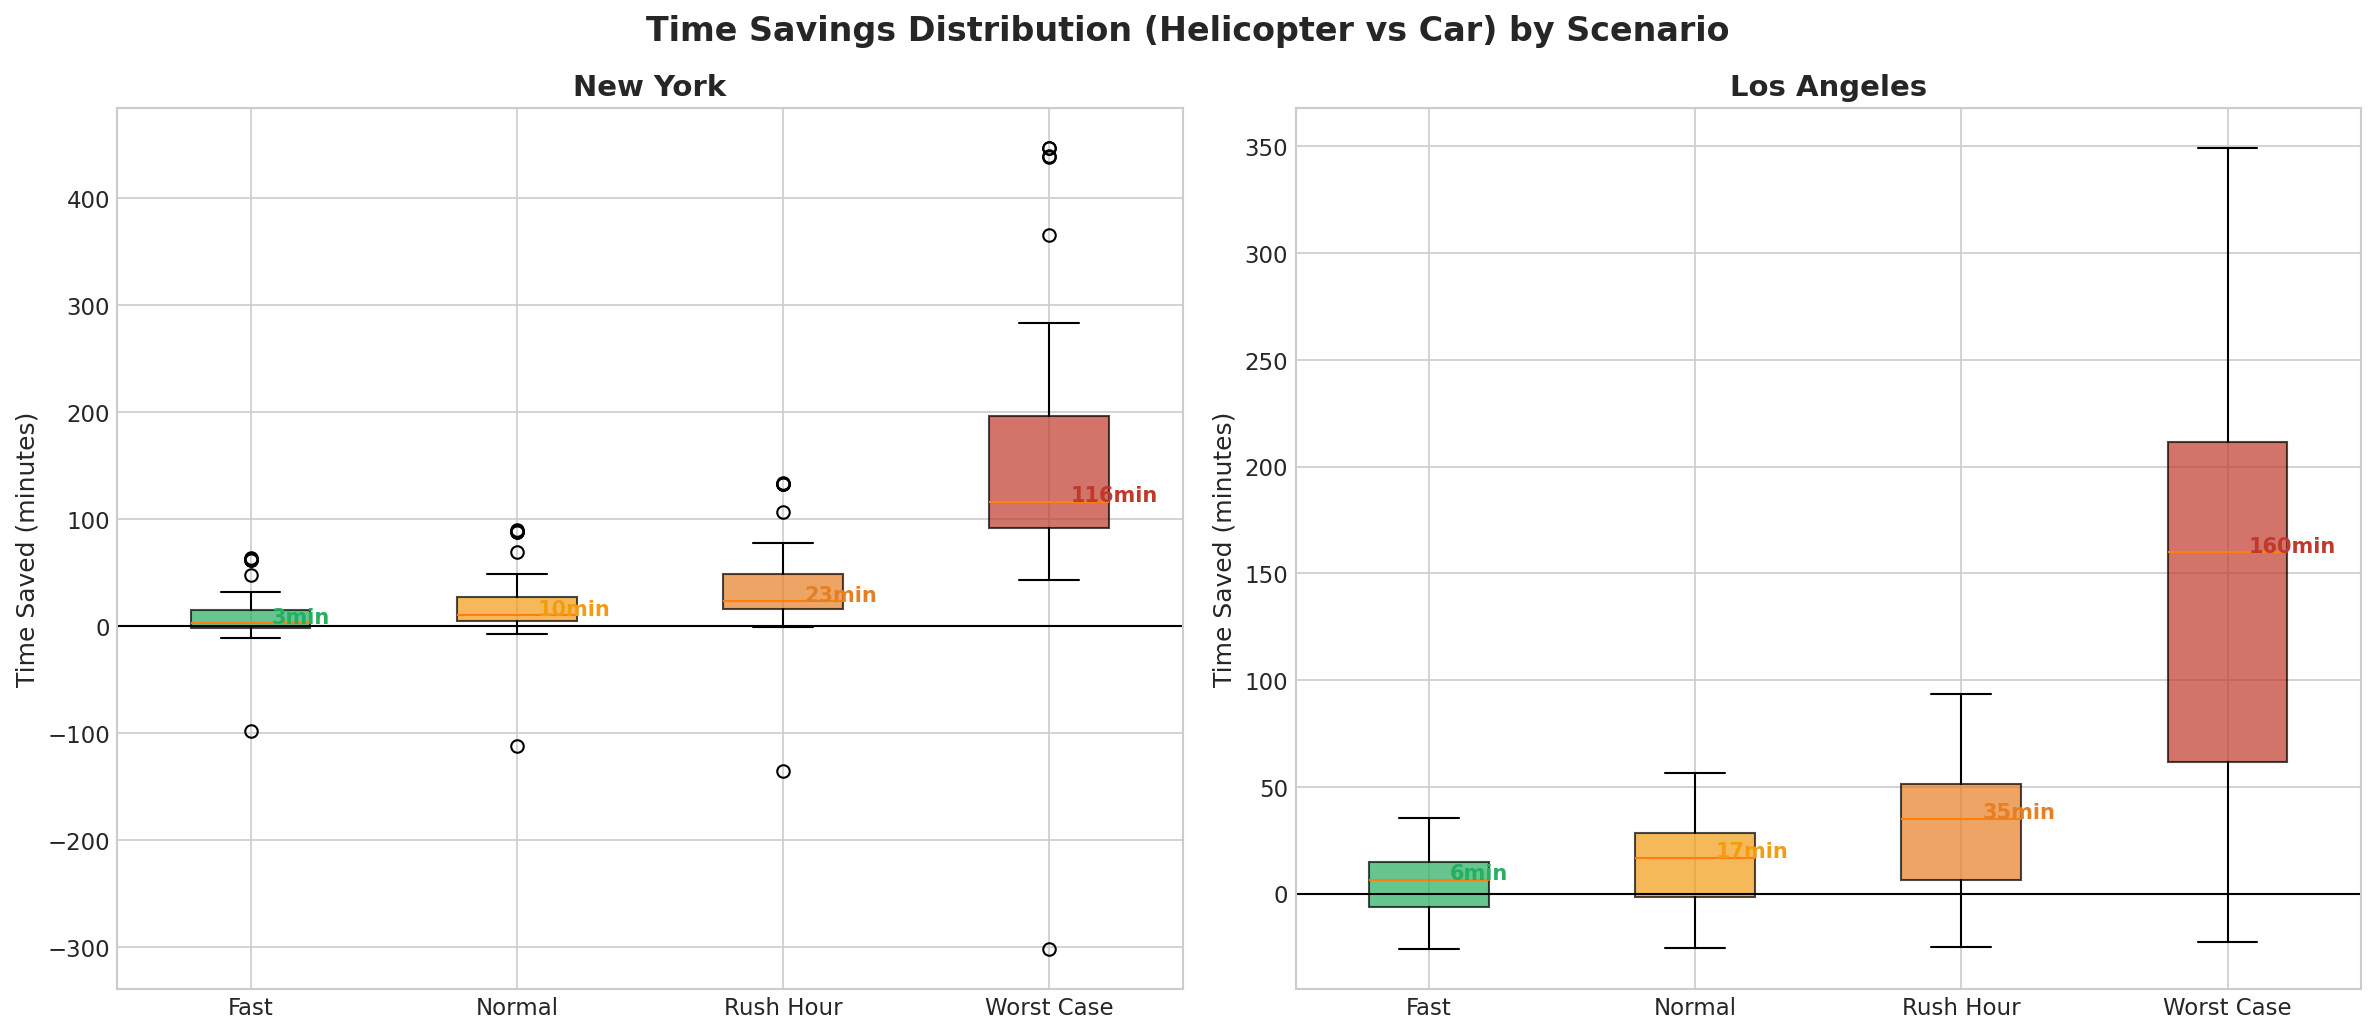
\includegraphics[width=\textwidth]{../comparison_charts_en/fig4_savings_boxplot.png}
\caption{Time Savings Distribution by Scenario (Boxplot)}
\label{fig:savings_boxplot}
\end{figure}

The boxplot reveals:
\begin{itemize}
    \item In \textbf{Fast} conditions, savings are minimal (median ~3 min)
    \item In \textbf{Worst Case}, median savings exceed 140 minutes
    \item LA shows slightly less variance due to more consistent traffic patterns
\end{itemize}

\subsection{Speed Analysis}

\begin{figure}[H]
\centering
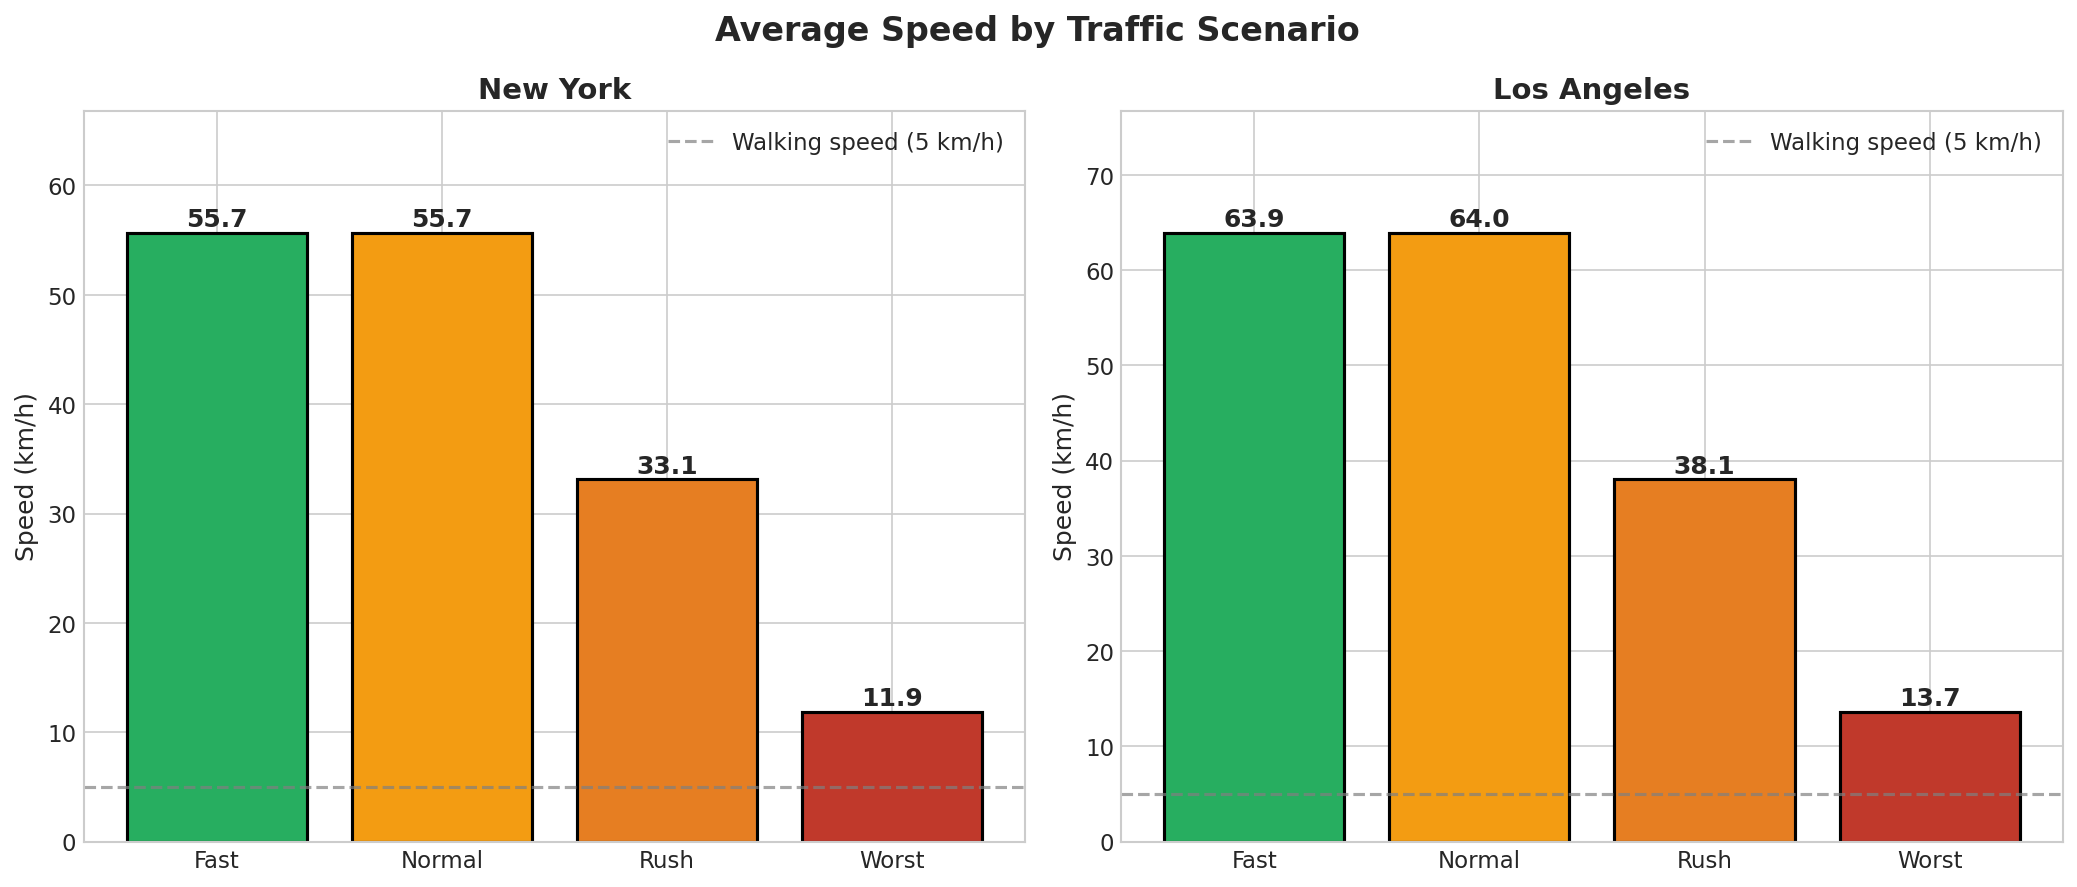
\includegraphics[width=\textwidth]{../comparison_charts_en/fig2_speed_comparison.png}
\caption{Average Speed by Traffic Scenario}
\label{fig:speed}
\end{figure}

Key findings:
\begin{itemize}
    \item \textbf{Worst Case Speed}: NY averages 12 km/h, LA averages 14 km/h
    \item Walking speed (5 km/h) is shown as reference
    \item During worst traffic, cars move only 2-3x faster than walking
\end{itemize}

\subsection{Time per 100 Meters}

\begin{figure}[H]
\centering
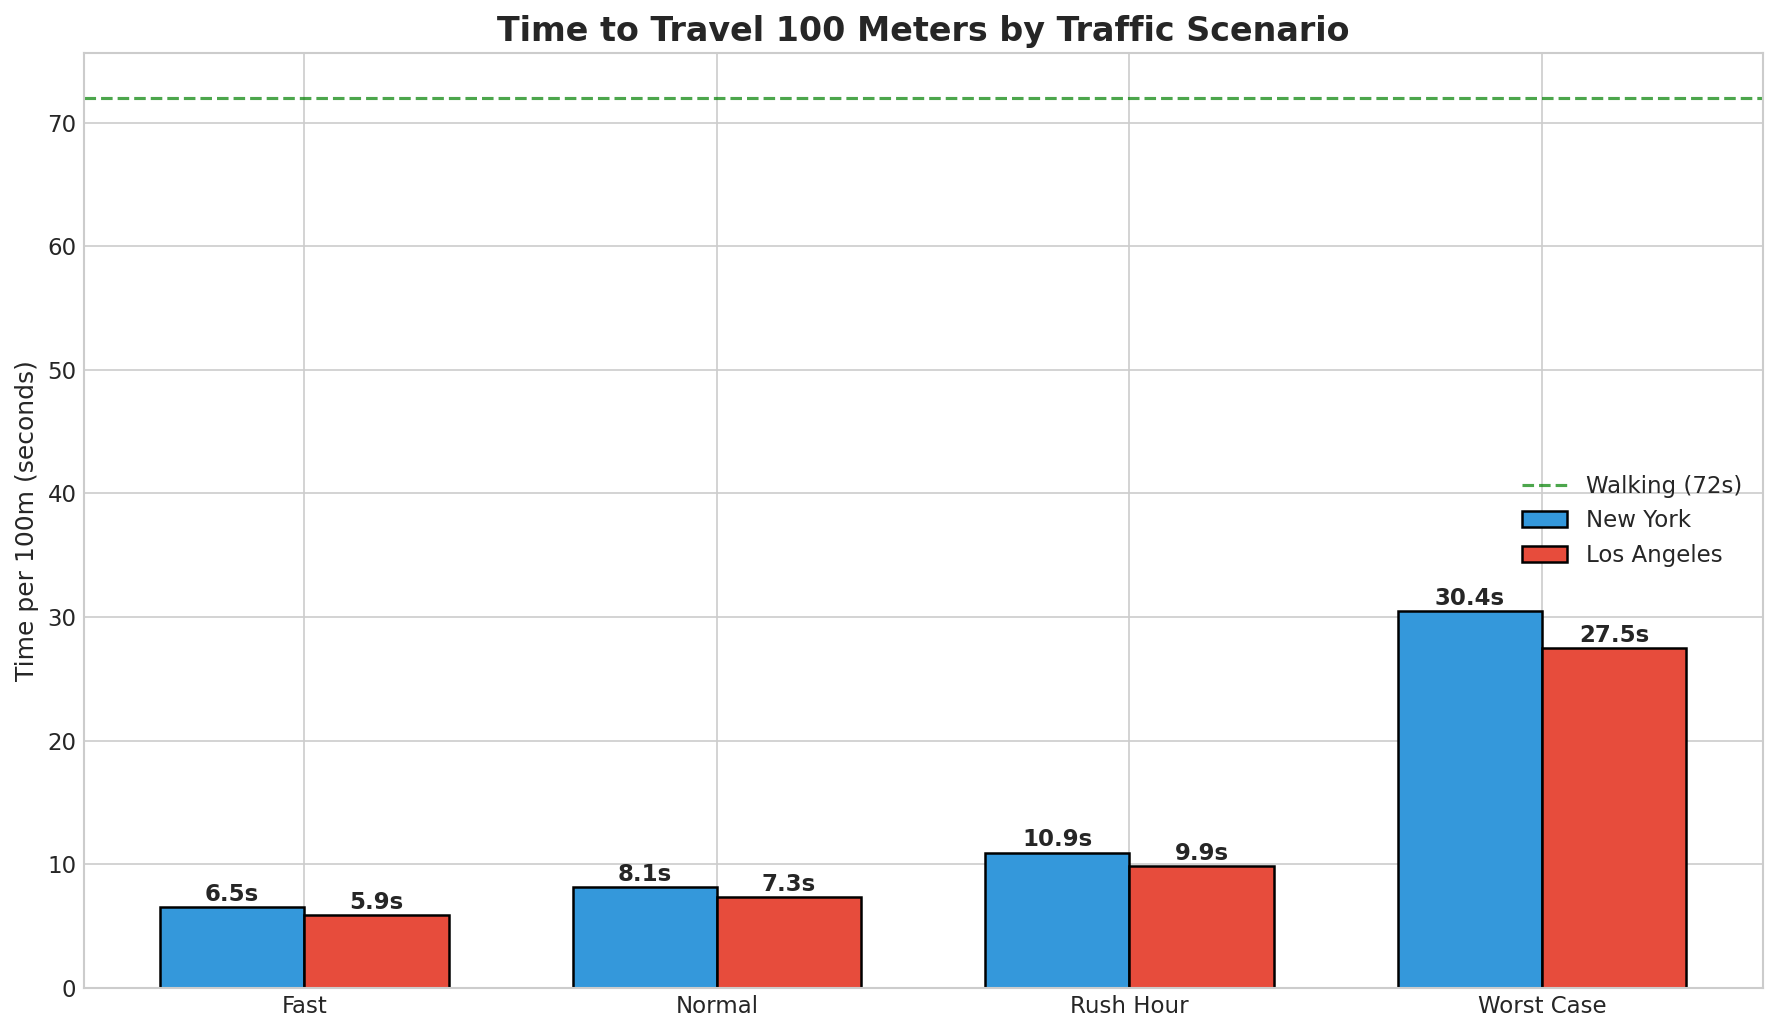
\includegraphics[width=\textwidth]{../comparison_charts_en/fig3_time_100m.png}
\caption{Time Required to Travel 100 Meters}
\label{fig:time_100m}
\end{figure}

In worst-case scenarios:
\begin{itemize}
    \item NY: ~30 seconds per 100m
    \item LA: ~26 seconds per 100m
    \item Walking pace (72 seconds per 100m) shown as reference
\end{itemize}

\subsection{Normal vs Worst Case Comparison}

\begin{figure}[H]
\centering
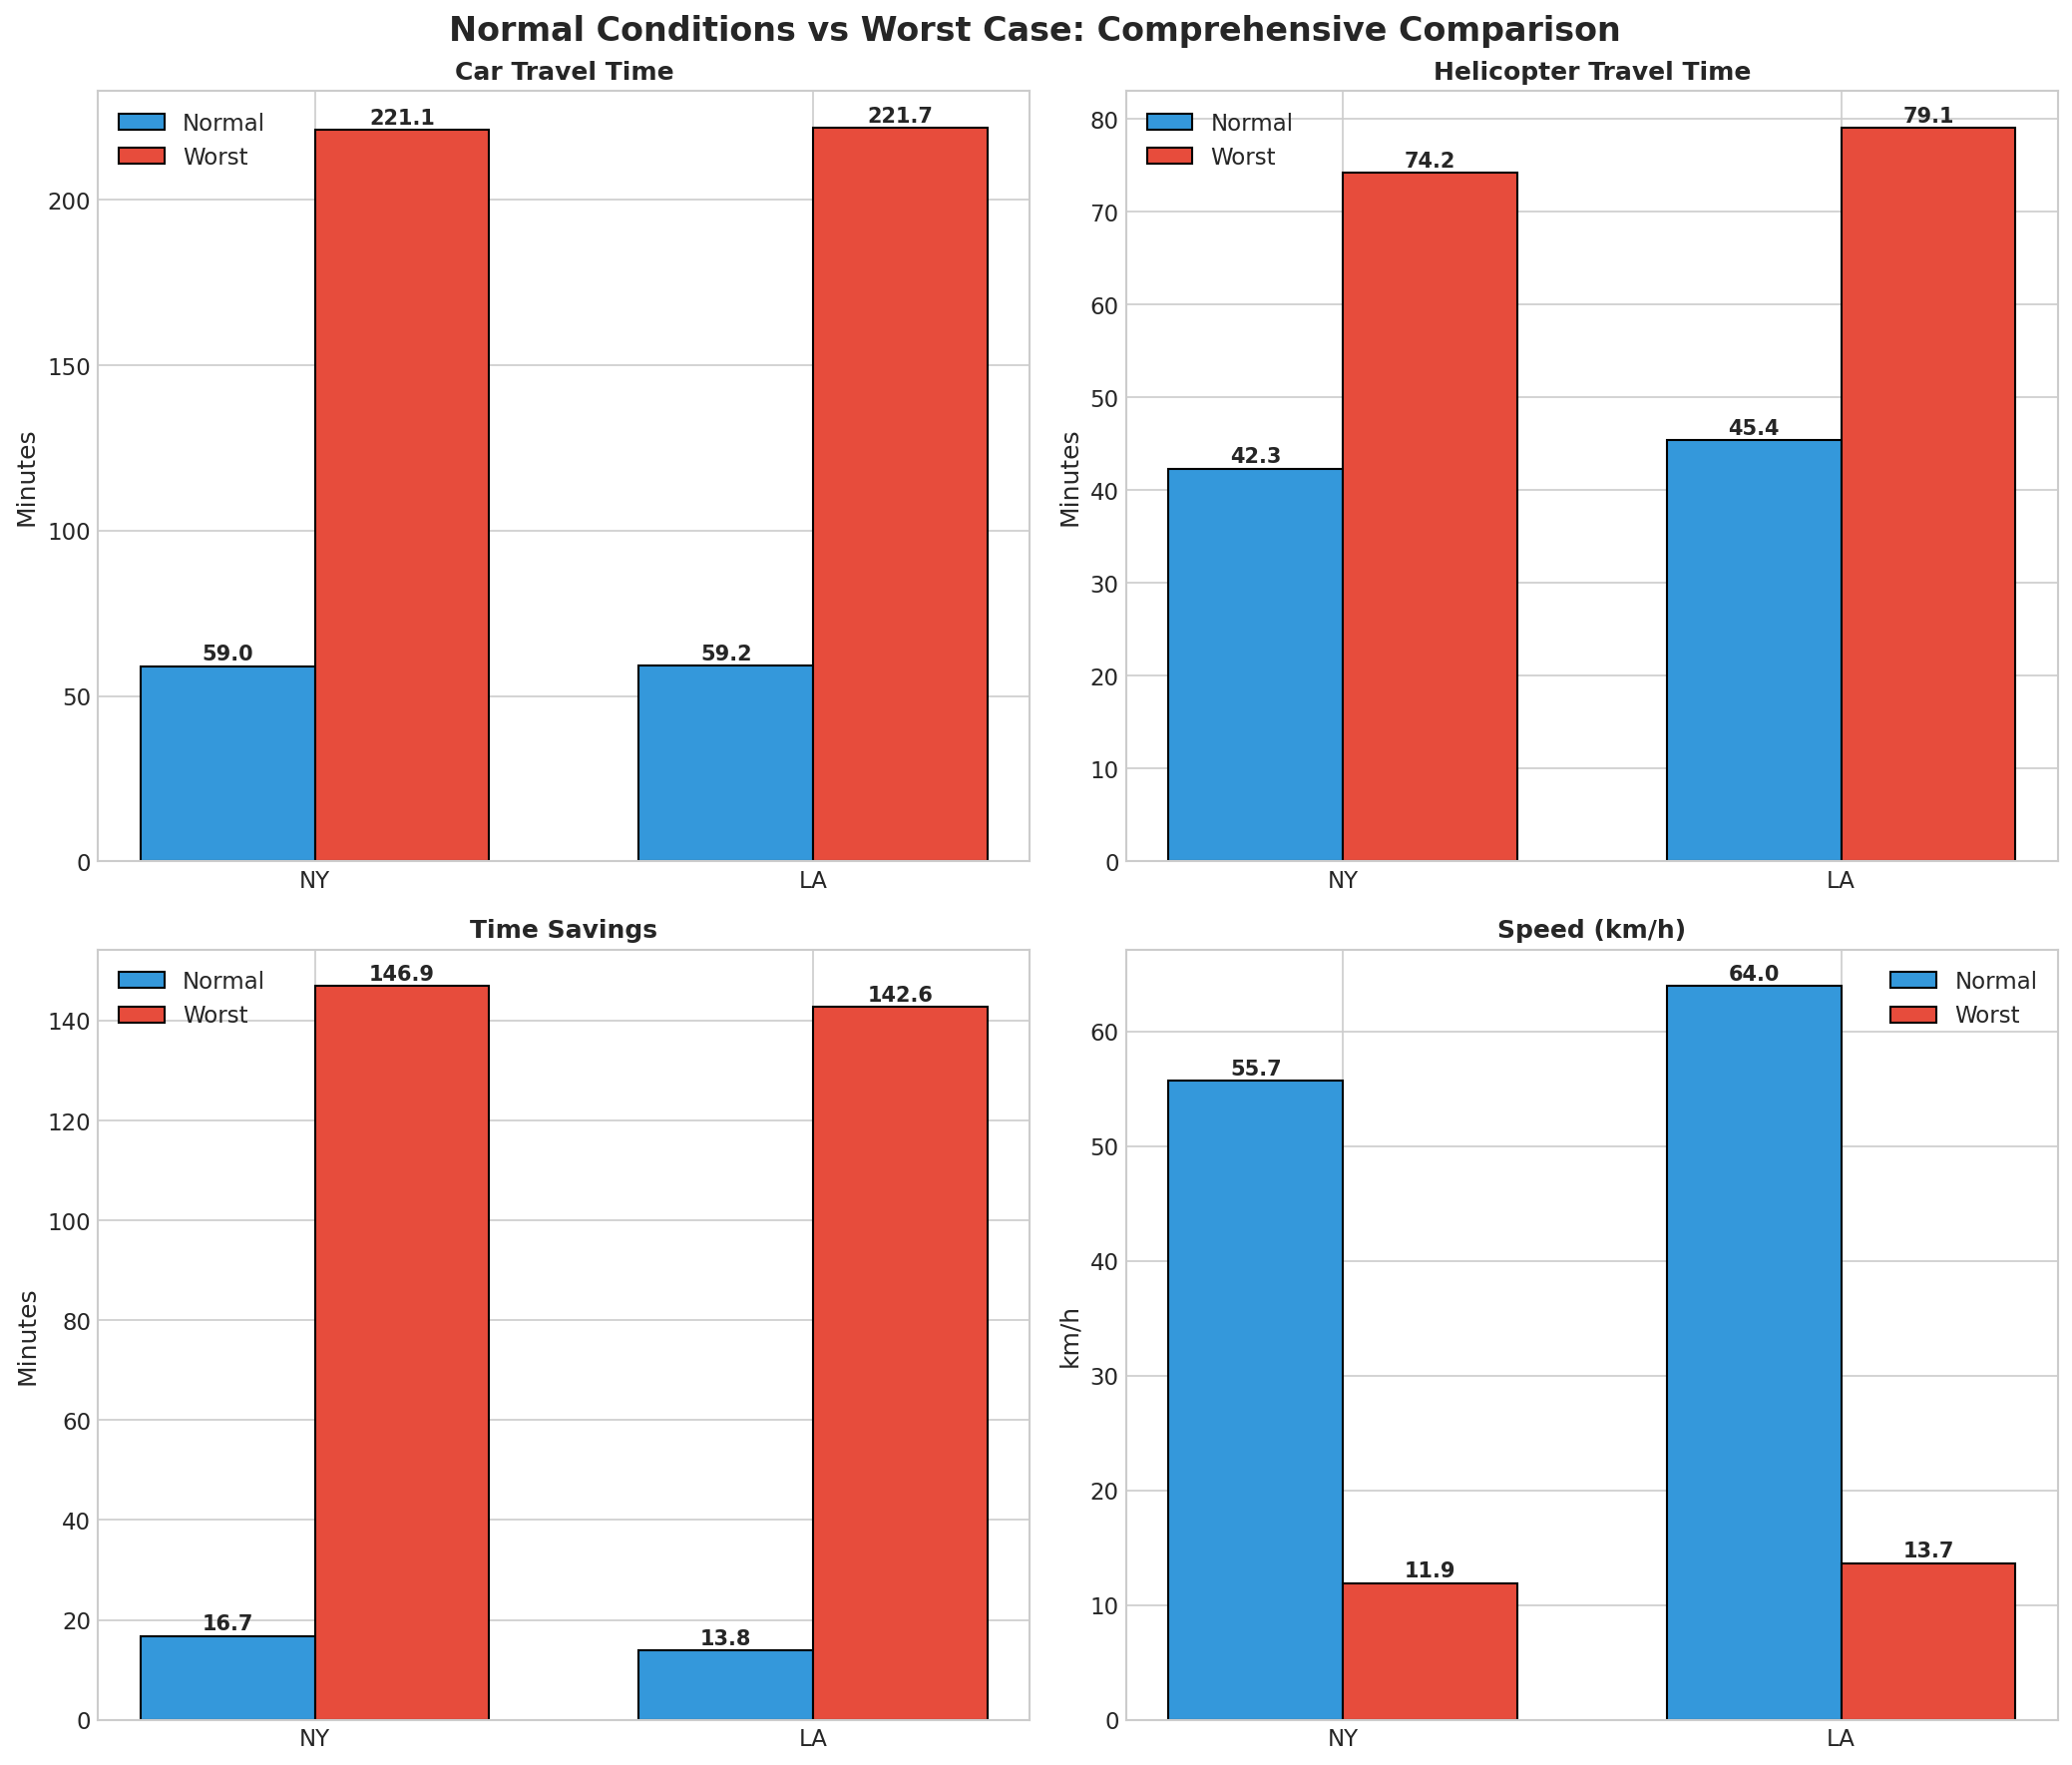
\includegraphics[width=\textwidth]{../comparison_charts_en/fig6_normal_vs_worst.png}
\caption{Direct Comparison: Normal Conditions vs Worst Case}
\label{fig:normal_vs_worst}
\end{figure}

This comparison highlights the dramatic difference between typical and worst-case scenarios:
\begin{itemize}
    \item Car travel time increases by \textbf{3.7x} from normal to worst
    \item Helicopter time increases by only \textbf{1.6x}
    \item Savings increase by \textbf{11x} (from 12 min to 145 min average)
\end{itemize}

\subsection{Multiplier Effect on Car Travel}

\begin{figure}[H]
\centering
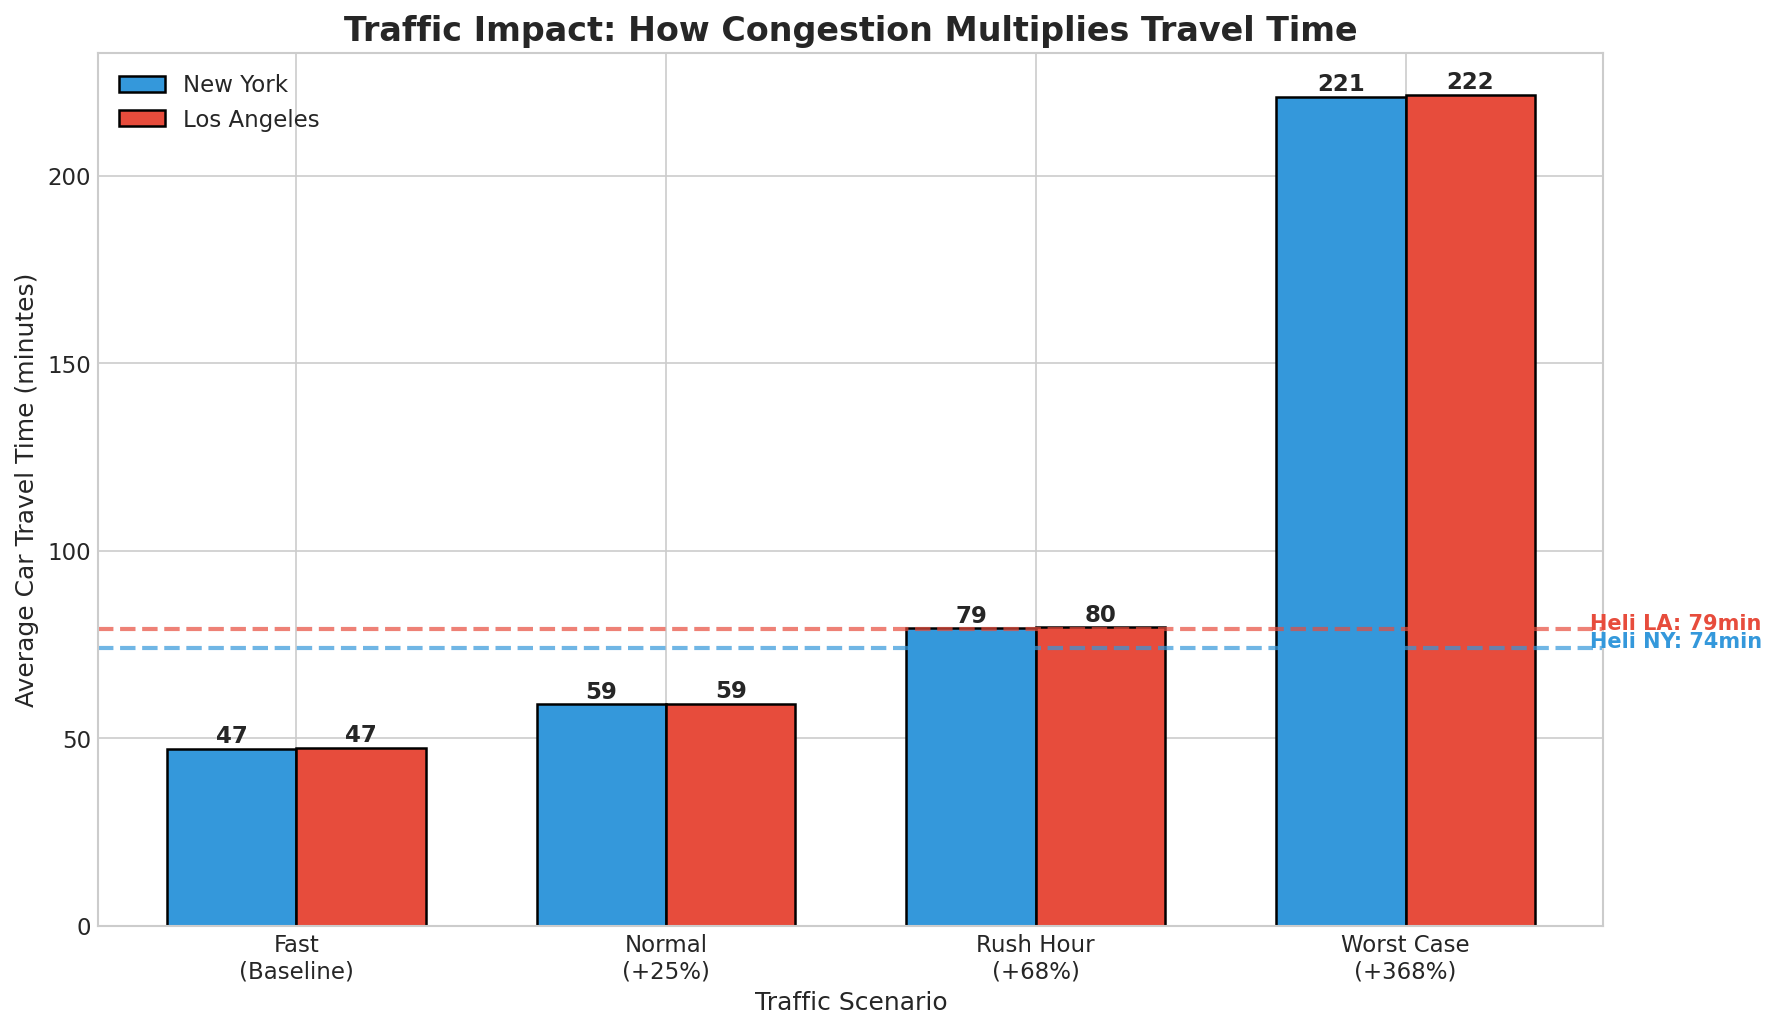
\includegraphics[width=\textwidth]{../comparison_charts_en/fig5_multiplier_effect.png}
\caption{How Traffic Congestion Multiplies Travel Time}
\label{fig:multiplier_effect}
\end{figure}

The horizontal dashed lines show helicopter times, which remain relatively stable across all scenarios because most of the helicopter journey (flight + fixed transfers) is unaffected by ground traffic.

\subsection{Savings Distribution Histogram}

\begin{figure}[H]
\centering
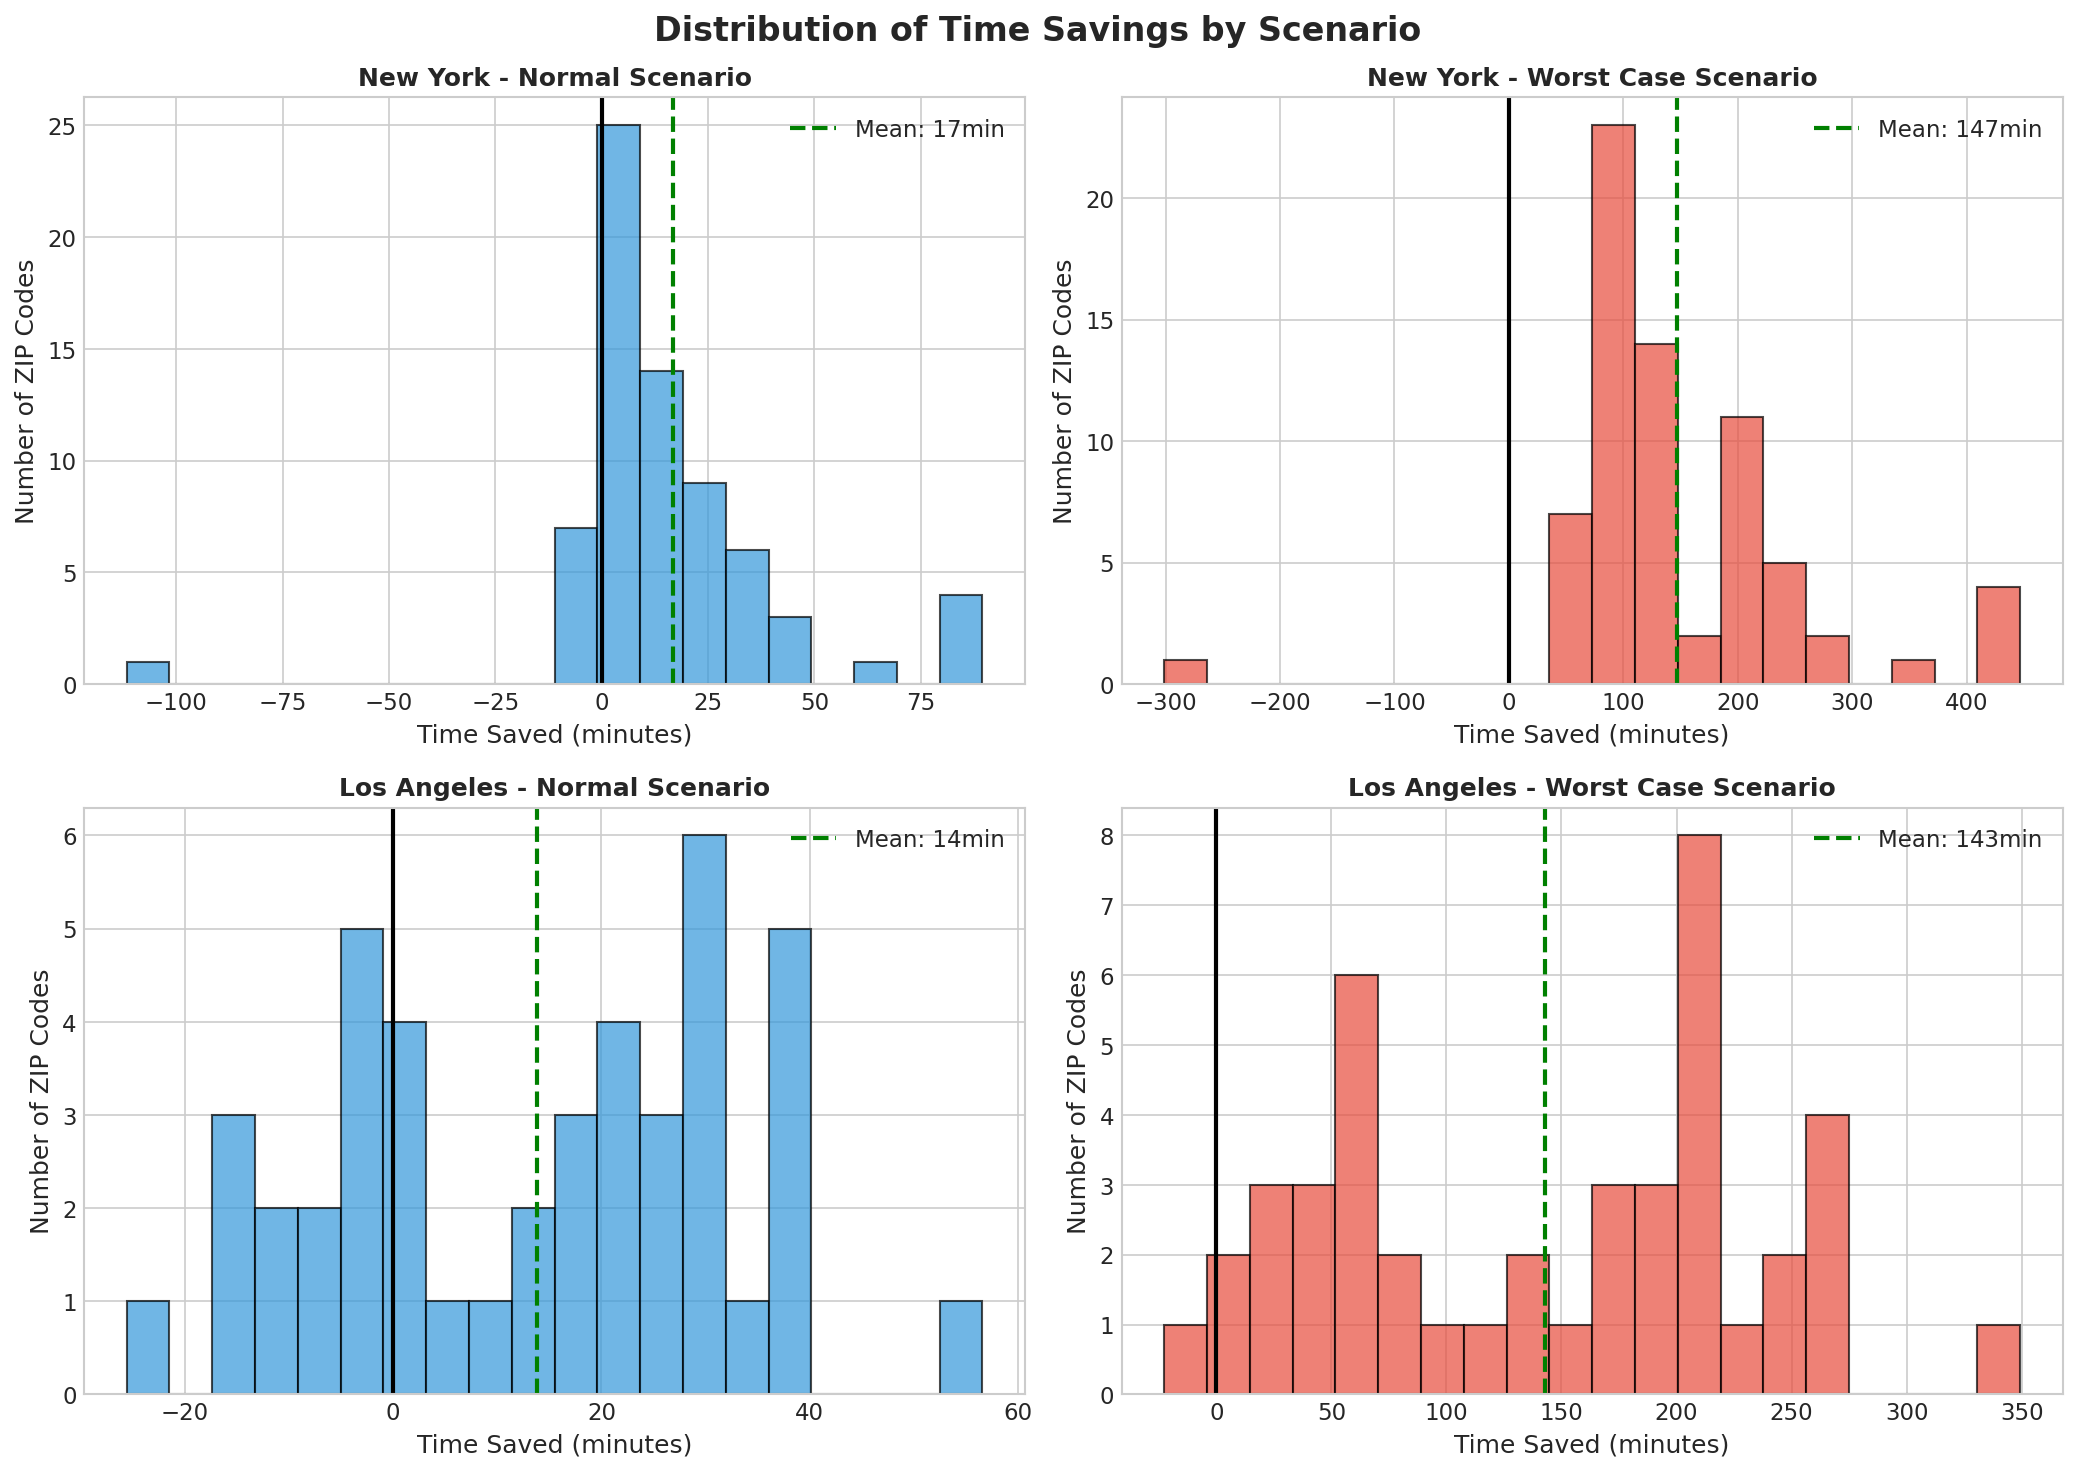
\includegraphics[width=\textwidth]{../comparison_charts_en/fig8_savings_histogram.png}
\caption{Distribution of Time Savings: Normal vs Worst Case}
\label{fig:histogram}
\end{figure}

Key observations:
\begin{itemize}
    \item \textbf{Normal scenario}: Savings centered around 10-15 minutes
    \item \textbf{Worst case}: Savings range from 100-200+ minutes
    \item Nearly all ZIP codes (99\%) show positive savings in worst case
\end{itemize}

\subsection{Time Breakdown Analysis}

\begin{figure}[H]
\centering
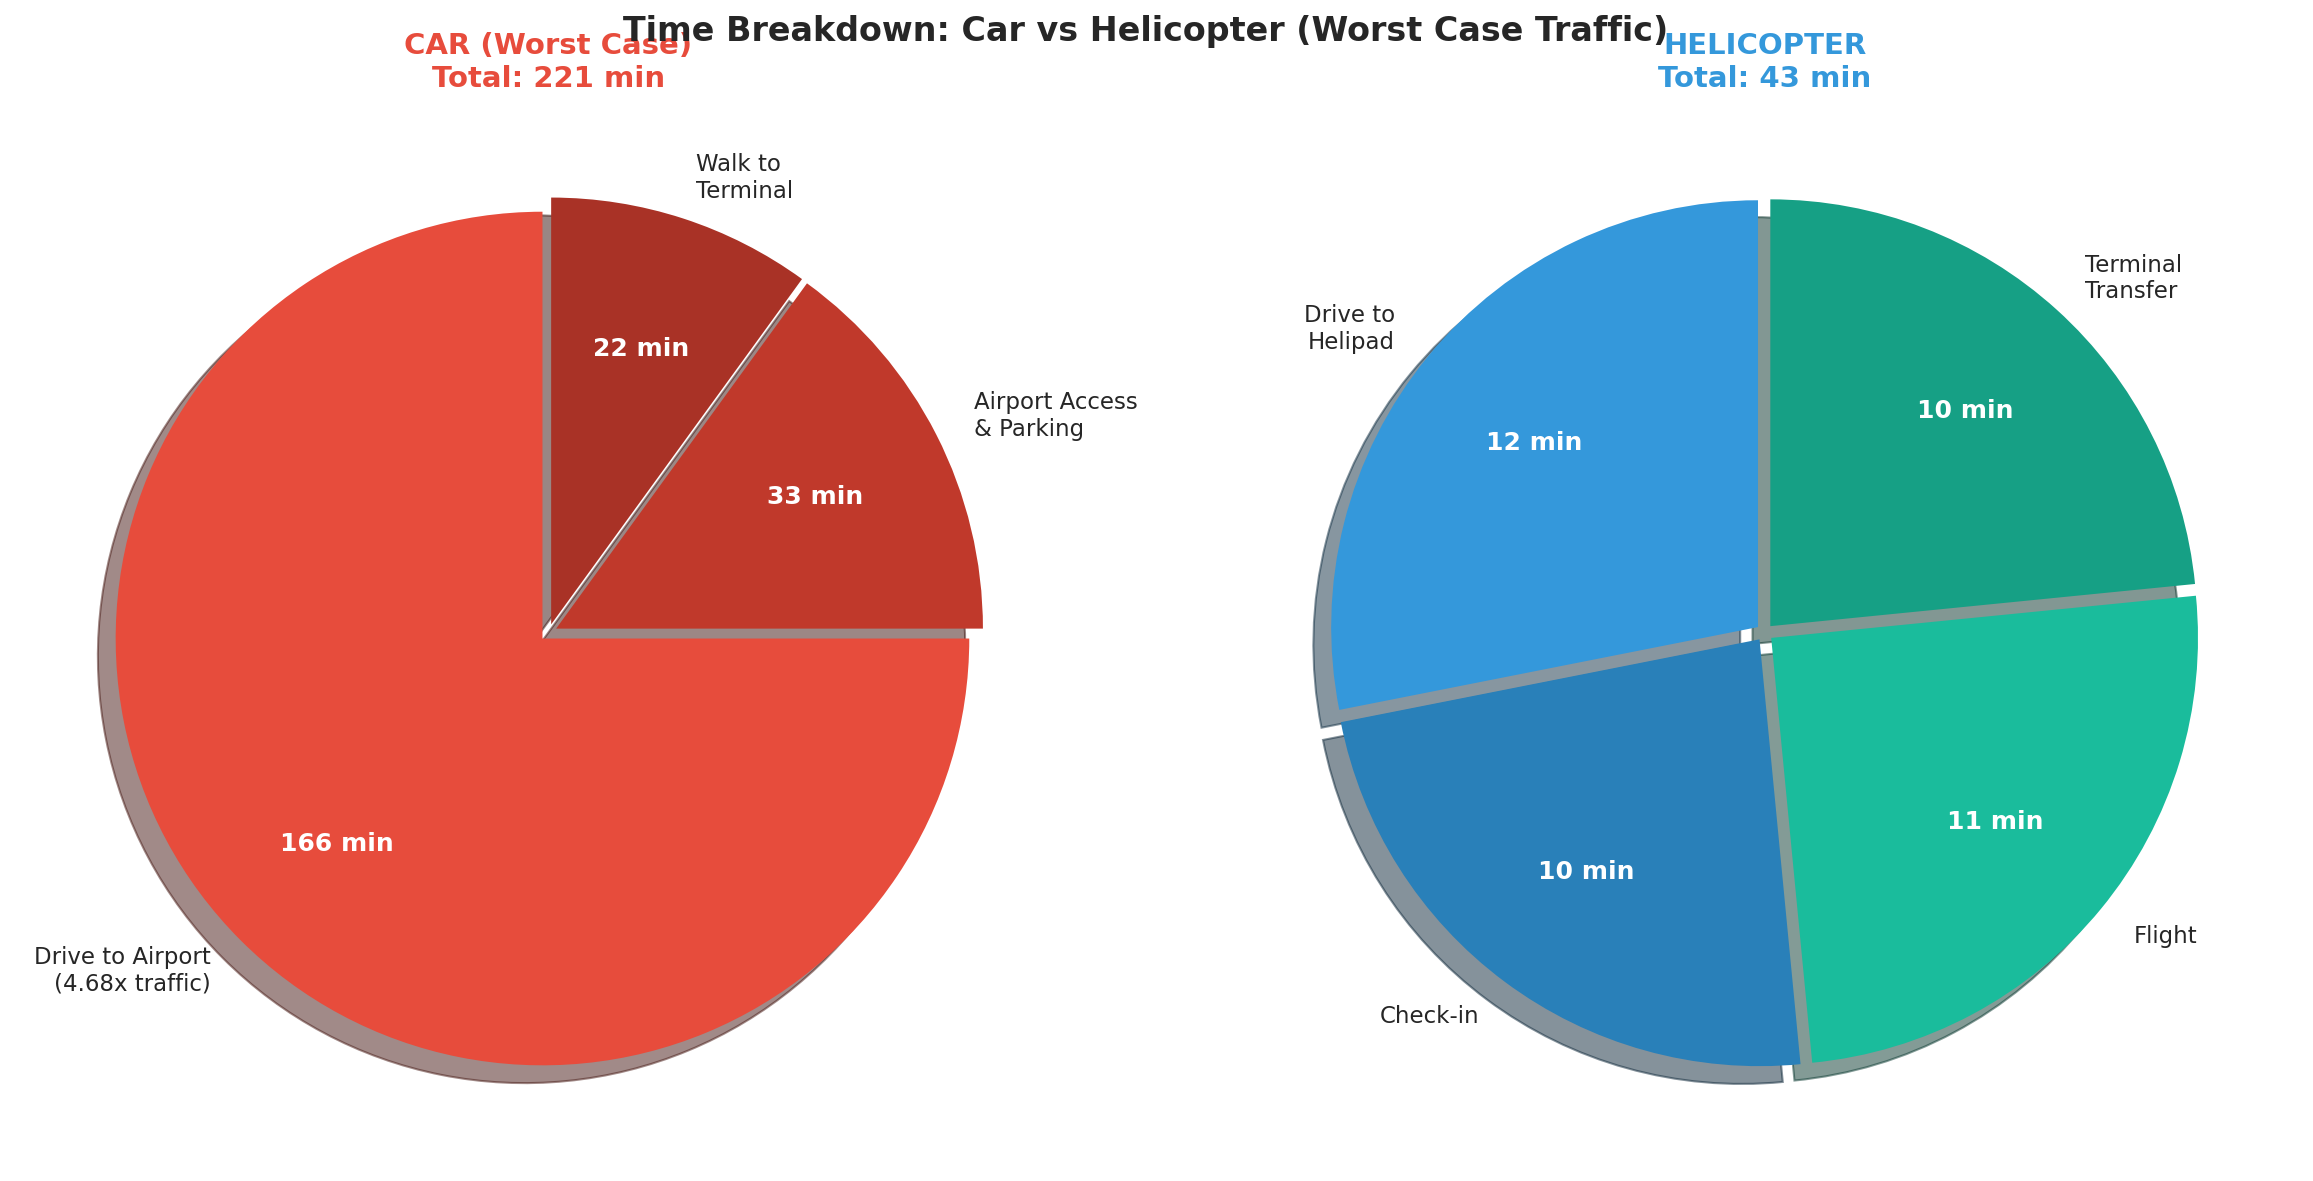
\includegraphics[width=0.9\textwidth]{../diagrams/time_breakdown_en.png}
\caption{Time Component Breakdown: Car vs Helicopter (Worst Case)}
\label{fig:breakdown}
\end{figure}

% ============================================================================
\section{Discussion}
% ============================================================================

\subsection{Key Findings}

\begin{enumerate}
    \item \textbf{Worst-case scenarios show dramatic helicopter advantage}: With 4.68x traffic multipliers, helicopter travel saves 2-3 hours compared to driving.
    
    \item \textbf{Speed degradation is severe}: In worst traffic, average speeds drop to 12-14 km/h---approaching bicycle speed.
    
    \item \textbf{Helicopter time stability}: Because the majority of helicopter journey time is fixed (check-in, flight, transfer), total time increases only modestly with traffic.
    
    \item \textbf{Manhattan shows strong advantage}: With helipads in Manhattan, residents avoid crossing congested bridges and tunnels.
\end{enumerate}

\subsection{Practical Implications}

\textbf{For Business Travelers}:
\begin{itemize}
    \item Helicopter service provides scheduling reliability
    \item Time savings of 2+ hours can mean the difference between making or missing flights
    \item Reduced stress and fatigue from avoiding traffic
\end{itemize}

\textbf{For Service Providers}:
\begin{itemize}
    \item Target marketing during known high-traffic periods
    \item Price premium justified during worst-case conditions
    \item Strategic helipad placement maximizes coverage
\end{itemize}

\subsection{Limitations}

\begin{itemize}
    \item Weather conditions may ground helicopter operations
    \item Helipad availability may be limited during peak demand
    \item Analysis assumes optimal helipad selection
    \item Cost differential not included in analysis
\end{itemize}

% ============================================================================
\section{Conclusions}
% ============================================================================

This comprehensive analysis demonstrates that helicopter transport provides significant time advantages over car travel, particularly during severe traffic conditions. Key conclusions:

\begin{enumerate}
    \item In \textbf{worst-case scenarios} (4.68x traffic), helicopter saves:
    \begin{itemize}
        \item New York: \textbf{147 minutes} (66\% reduction)
        \item Los Angeles: \textbf{143 minutes} (64\% reduction)
    \end{itemize}
    
    \item The advantage increases exponentially with traffic severity
    
    \item \textbf{99\% of ZIP codes} show helicopter advantage during worst traffic
    
    \item Ground speeds during worst traffic (~12 km/h) make helicopter the only viable option for time-sensitive travel
\end{enumerate}

% ============================================================================
\section{Summary Statistics}
% ============================================================================

\begin{figure}[H]
\centering
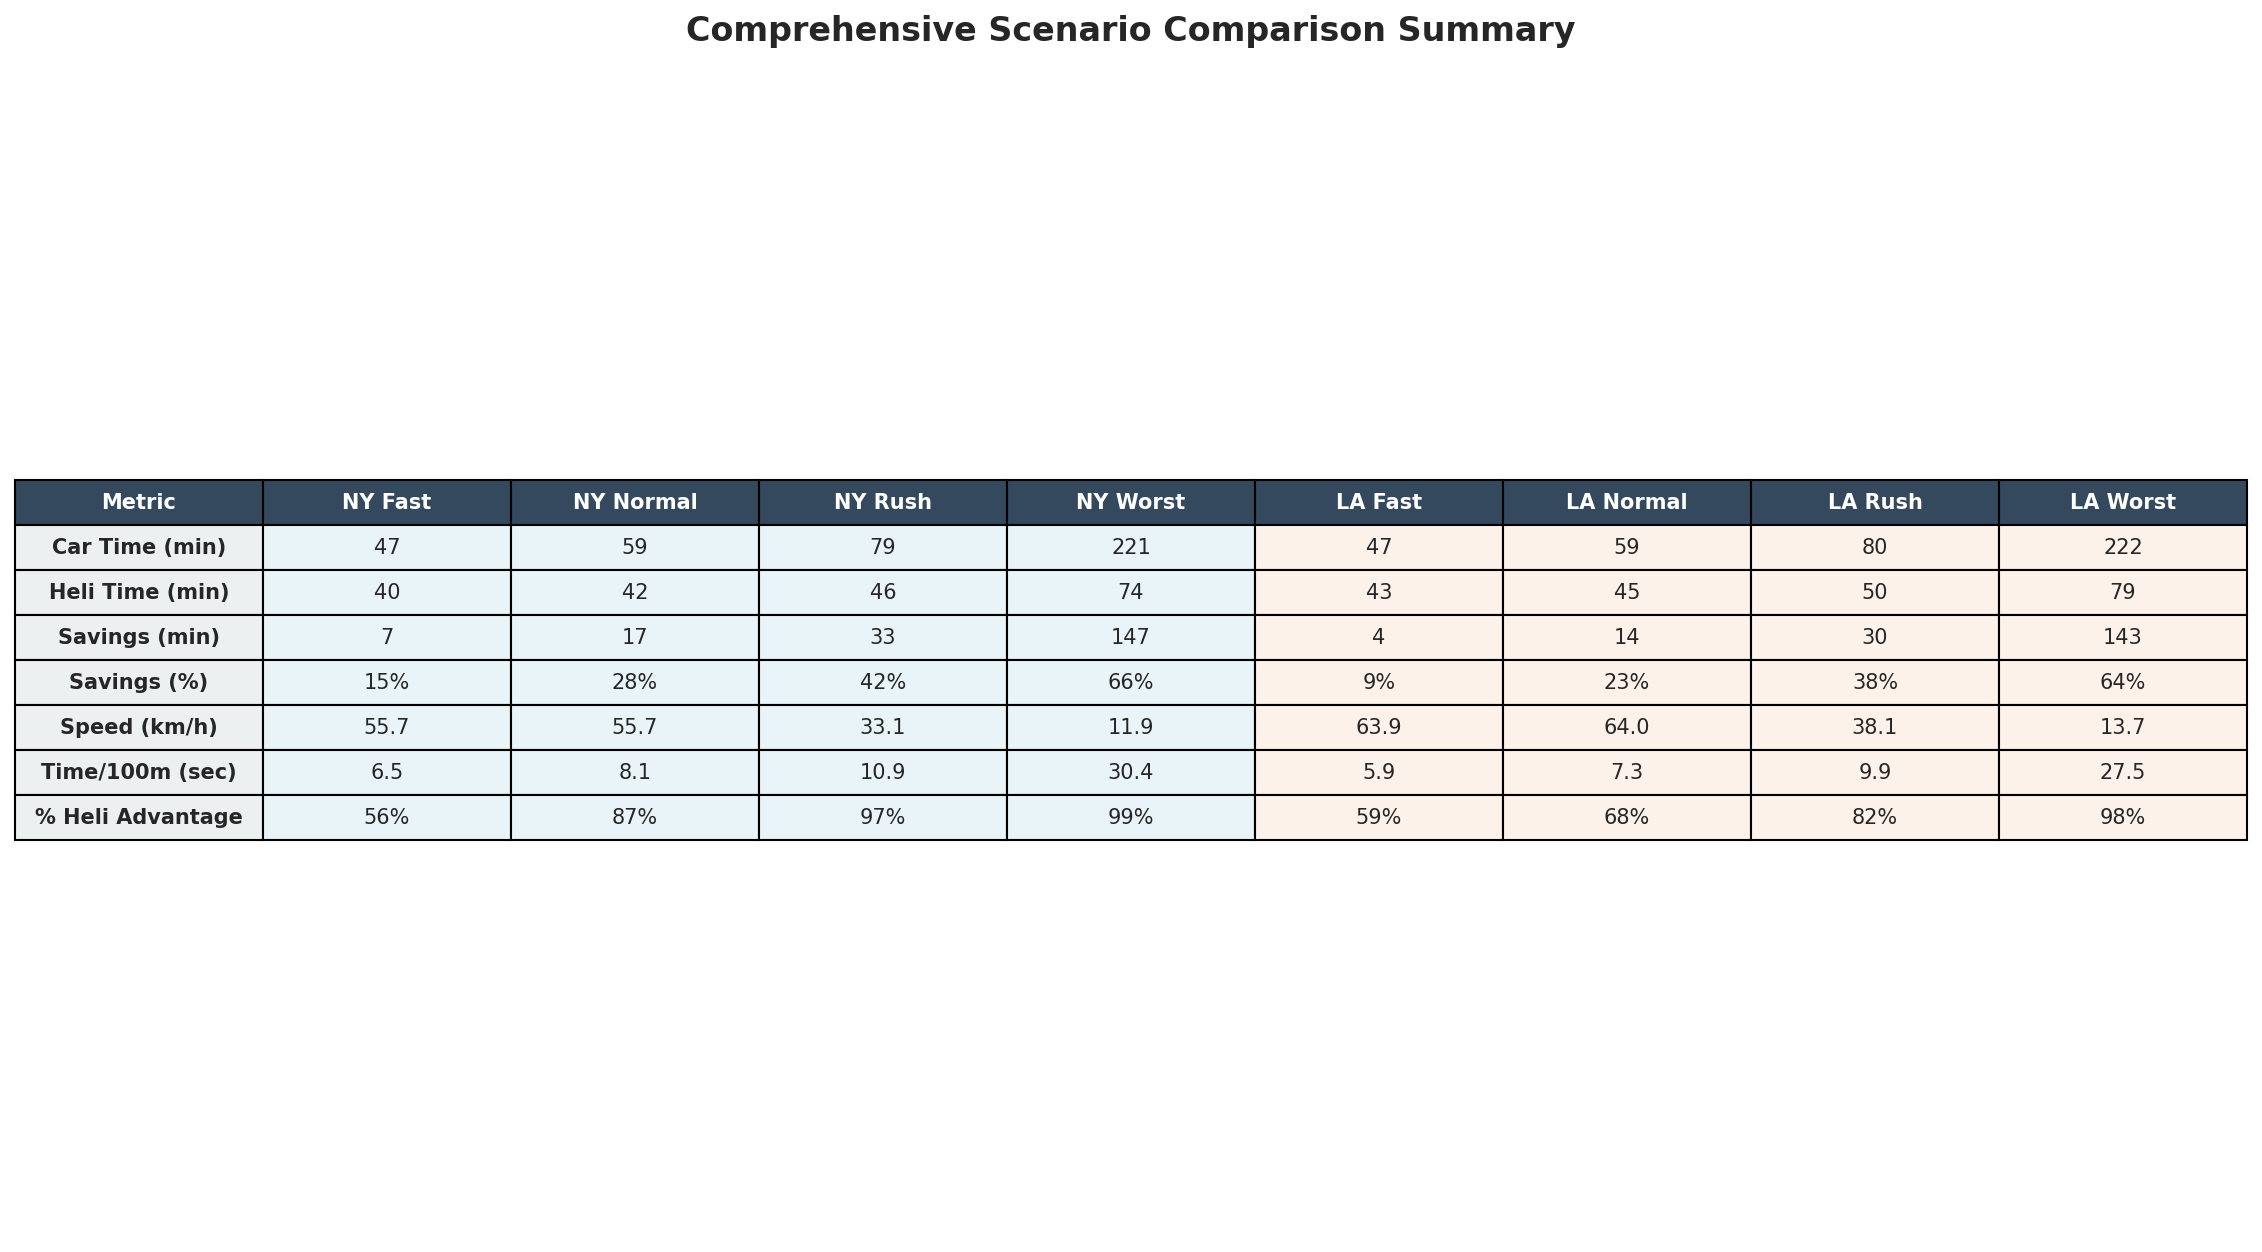
\includegraphics[width=\textwidth]{../comparison_charts_en/fig7_summary_table.png}
\caption{Complete Summary Statistics Table}
\label{fig:summary}
\end{figure}

% ============================================================================
\appendix
\section{Data Sources}
% ============================================================================

\begin{itemize}
    \item \textbf{Traffic Data}: Google Traffic API (Pessimistic Duration)
    \item \textbf{Routing}: OSRM (Open Source Routing Machine)
    \item \textbf{Helipad Data}: FAA Airport/Heliport Database
    \item \textbf{ZIP Code Data}: Top 10\% wealthiest ZIP codes by income
\end{itemize}

\section{Technical Parameters}

\begin{table}[H]
\centering
\caption{Analysis Parameters}
\begin{tabular}{ll}
\toprule
\textbf{Parameter} & \textbf{Value} \\
\midrule
Helicopter cruise speed & 200 km/h \\
Helipad check-in time & 10 minutes \\
Airport transfer time & 10 minutes \\
Number of NY ZIP codes & 70 \\
Number of LA ZIP codes & 44 \\
Manhattan ZIP codes & 27 \\
Total heliports considered & 65 (34 NY, 31 LA) \\
\bottomrule
\end{tabular}
\end{table}

\end{document}

